\documentclass{article}
\usepackage{graphicx} % Required for inserting images
\usepackage{tabto}

\title{BPC PCB Overview}
\author{Noah Rothgaber and John Brann}
\date{September 2024}

\begin{document}

\maketitle
\section{Introduction}

In order to assist in the assembly of our Gripper, we chose to design a Printed Circuit Board (PCB). Using a PCB to control the electronics, instead of options like a breadboard, helps the assembler avoid wiring numerous jumpers, accidentally connecting incorrect pin pairs, and dealing with complex wiring diagrams. Additionally, jumper wires can fray and cause hard-to-diagnose errors, so minimizing their use reduces the chances of such issues and makes troubleshooting more straightforward.\\

Within this document, we will be going over the construction of the board, its various components, and their functionality.\\

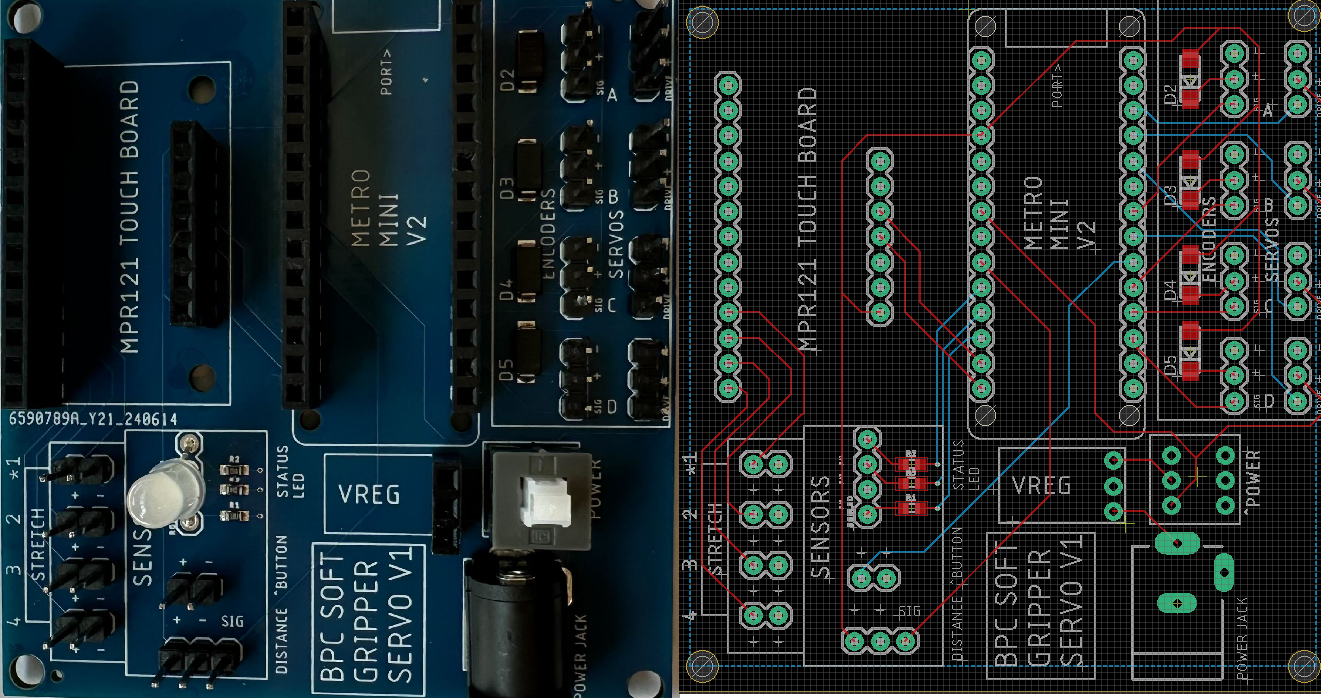
\includegraphics[]{Images/Combined.png}
\section{Metro Mini V2 and MPR121}
In the top/center - left/center of the PCB lie the female headers for the two main boards we use for the Gripper. The center-most headers are used to connect the Adafruit Metro Mini V2  \textit{(Metro for short)}, which is a powerful Arduino-based micro-controller and the core of our PCB. The left-most headers are used for the Adafruit MPR121, a capacitive touch sensor breakout board capable of capturing data from touch/stretch sensors. The MPR121's output is connected to our Metro via two traces running from the SDA and SCL pins of the MPR121 to the A5 and A4 pins.\\

\begin{center}
    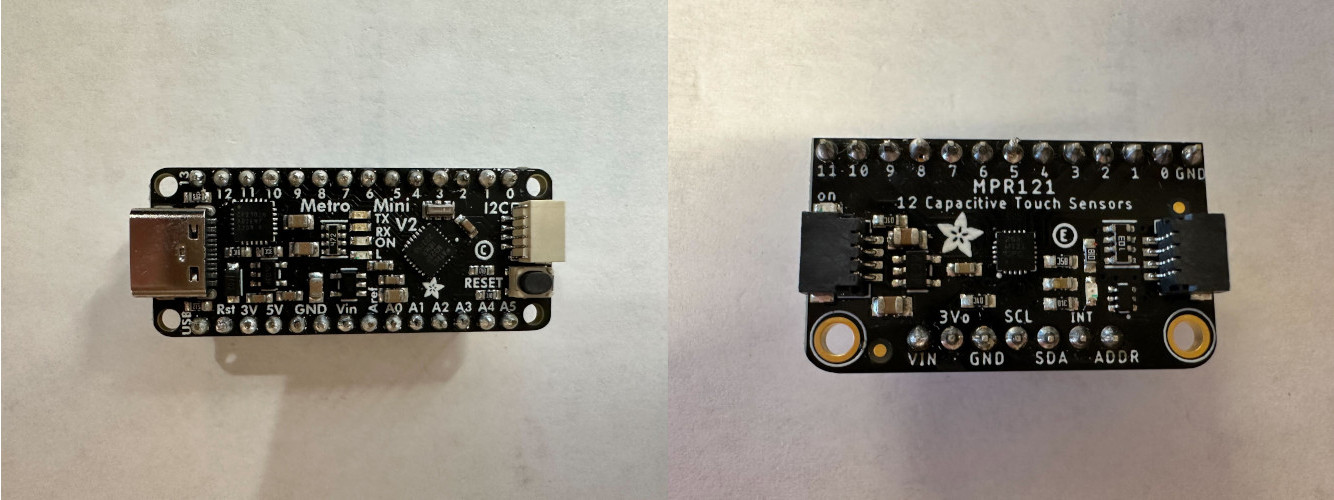
\includegraphics[scale=0.25]{Images/metroandmpr.jpg}
    \\[1ex] % Adjusting spacing
    \textit{$\>$ $\>$ $\>$ $\>$ $\>$ Adafruit Metro Mini V2 \tab Adafruit MPR121}
\end{center}
\section{Servo/Encoder Headers}
Our PCB is equipped to handle up to four Servos and their Encoders. Both the Encoders and the Servos are connected via female connectors to the male pin headers located on the top-right corner of the PCB. The sections are labeled with + and - symbols to indicate the proper alignment of the connectors. As a precaution, the Encoder headers do not run directly to the power source but instead are run through diodes, which ensure that the connector is not flipped upside down (which could cause reverse current and damage the PCB/Components). The Servos are labeled A, B, C, D and are connected (via traces) to pins 11, 10, 9, and 6. The Encoders are labeled the same as the Servos but are instead connected to pins 7, 4, 3, 2 (also via traces).\\
\begin{center}
    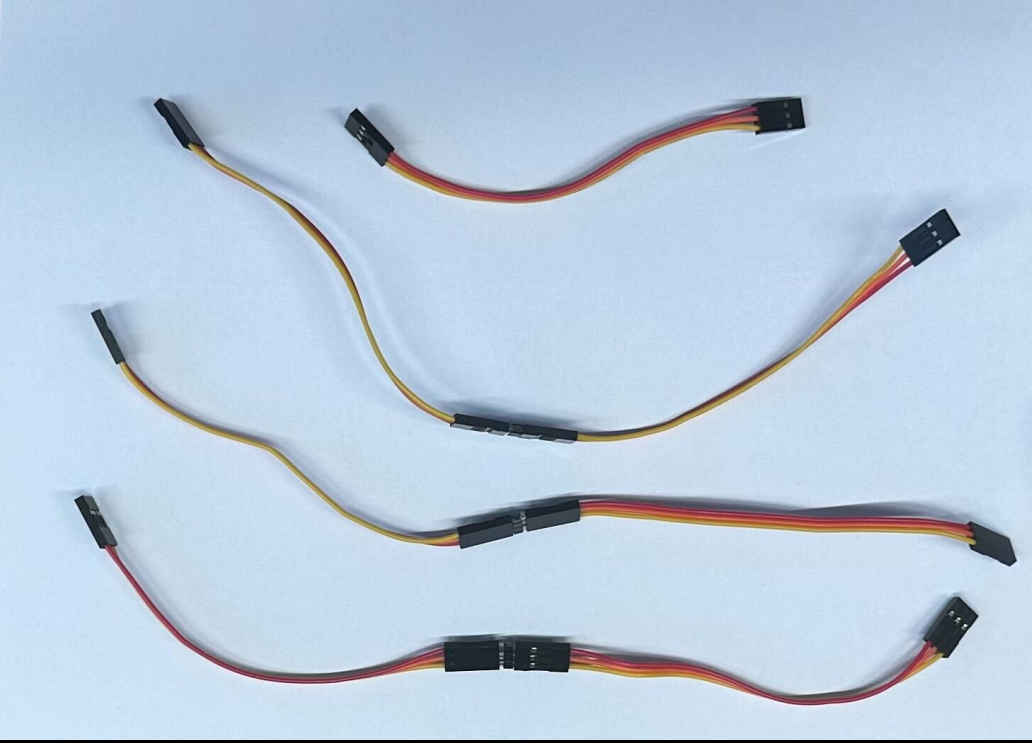
\includegraphics[scale=0.17]{Images/EncoderJumpersCropped.png}
    \\[1ex] % Adjust spacing if needed
    \textit{Note: The female connector is built directly into the Servos we provide, but the Encoders require jumper wires to be able to connect (shown above).}
\end{center}
\section{Sensors}
Our PCB supports up to four capacitive stretch sensors, one Push Button, and one Ultrasonic Distance Sensor as its input devices. The stretch sensors are used to control the closing of our Gripper either with a threshold we set in the code, or the degree of stretch the sensor is pulled to. The Distance Sensor functions nearly identically to the stretch sensor with its proportional or threshold control of the Gripper but is instead measuring the distance from the sensor to an object. The Push Button can be used to move the Gripper to the fully open position.\\

The male header connectors for these accessories are located at the bottom left of the PCB in the section labeled "Sensors." The four capacitive touch sensors are connected to the MPR121's 11, 10, 9, and 8 pins (via traces). The Push Button and the Ultrasonic Distance Sensor are connected to the Metro (via traces) on pins 5 and 14, respectively.\\
\begin{center}
    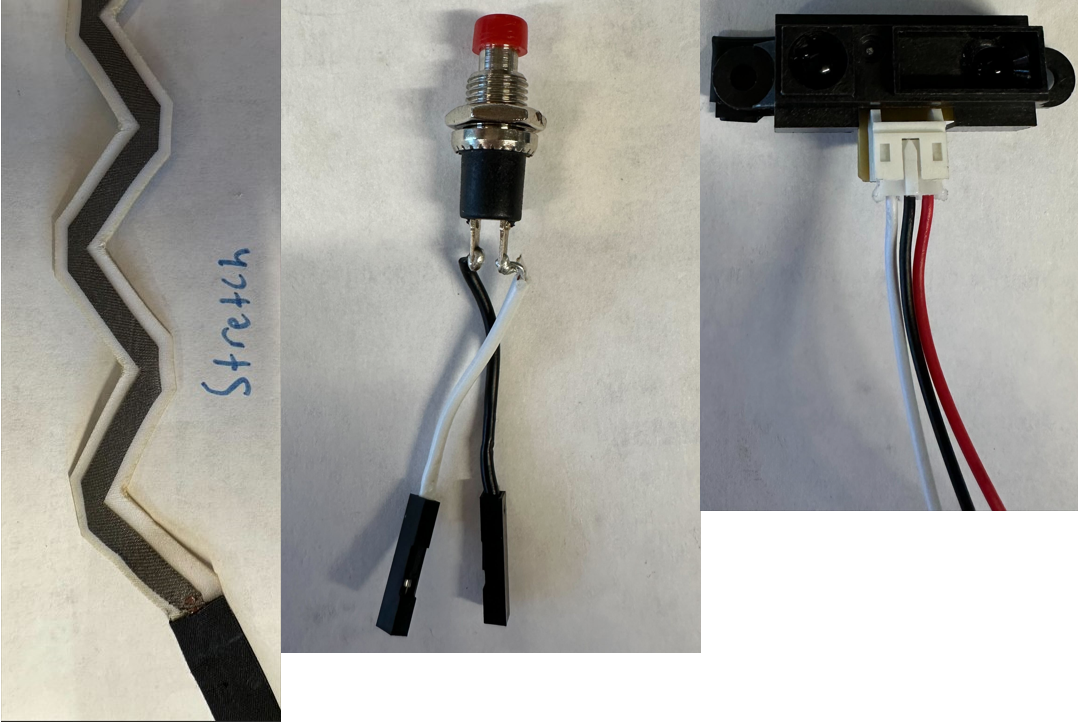
\includegraphics[scale=1]{Images/AllSensors.png}
    \\[1ex] % Adjust spacing if needed
    \textit{From left to right: Stretch Sensor, Push Button, Distance Sensor}
\end{center}

\section{LED}
Within the same section as the Sensors, we've included an RGB LED. This LED is used to communicate the status of the Gripper to the user via our Arduino C program. The Blue and Green pins are connected to 100$\Omega$ resistors, while the Red pin of the LED is attached to a single 180$\Omega$ resistor. These resistors are then connected to the Metro (via traces) on pins A1, A2, A3. 
\begin{center}
    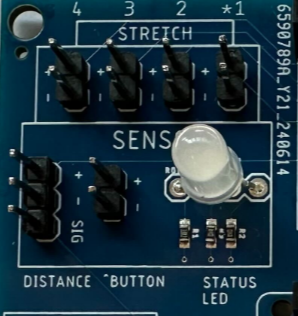
\includegraphics[scale=.80]{Images/SensorsSection.png}
    \\[1ex] % Adjust spacing if needed
    \textit{Sensors Section with LED}
\end{center}
\section{Power}
The PCB is powered using a 2.1mm DC Power Jack, a 9V DC adapter (separate from the PCB), a Pololu 5V Voltage Regulator, and a toggling Power Button. The Metro, MPR121, Servos, Encoders, LED, and Distance Sensor all require 5V of power, so dropping the voltage to approximately 5V allows the whole system to run. The DC Jack is connected to the Voltage Regulator, and the Voltage Regulator is connected to the Power Button, which allows the user to power off and on the Gripper. \\
\begin{center}
    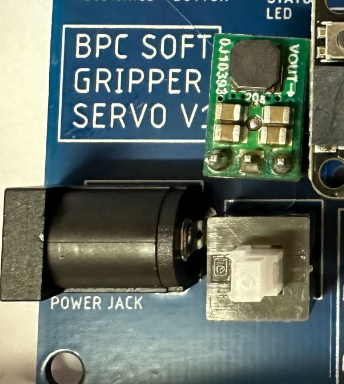
\includegraphics[scale=.5]{Images/PowerSection.png}
    \\[1ex] % Adjust spacing if needed
    \textit{The DC Power Jack, Voltage Regulator, and Power Button}
\end{center}
\end{document}
